\documentclass[12pt,a4paper]{scrartcl}
\usepackage[utf8]{inputenc}
\usepackage[english,russian]{babel}
\usepackage{indentfirst}
\usepackage{misccorr}
\usepackage{graphicx}
\usepackage{amsmath}
\usepackage{hyperref}
\usepackage{float}

\usepackage{graphicx}
\graphicspath{{/}}
\DeclareGraphicsExtensions{.pdf,.png,.jpg,.jpeg}

\begin{document}
	
	\section{Оптимальное асимметричное шифрование с дополнением (OAEP)}
	
	OAEP (англ. Optimal Asymmetric Encryption Padding, Оптимальное асимметричное шифрование с дополнением) — схема дополнения, обычно используемая совместно с какой-либо односторонней функцией с потайным входом (например RSA или функции Рабина) для повышения криптостойкости последней. OAEP предложено Михиром Белларе и Филлипом Рогавэем, а его применение для RSA впоследствии стандартизировано. Использование этой схемы отсекает много рассмотренных атак, поэтому на практике она сейчас идёт в духе "общеобязательной".
	
	\subsection{Схема OAEP}
	
	Классическая схема OAEP представляет собой двухъячеечную сеть Фейстеля, где в каждой ячейке данные преобразуются с помощью криптографической хеш-функции. На вход сеть получает сообщение с дописанными к нему проверяющими нулями и ключ — случайную строку.
	
	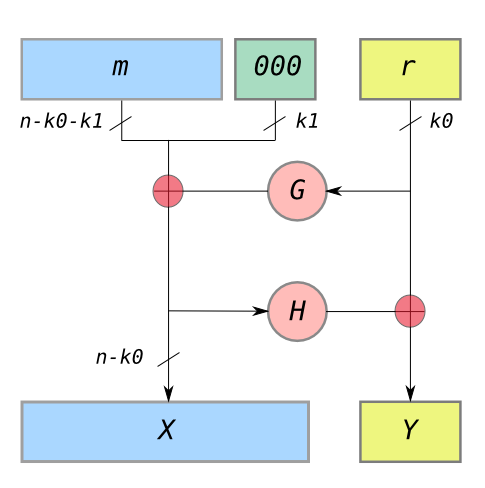
\includegraphics[scale=0.7]{oaep}
	
	В схеме используются следующие обозначения:
	
	\begin{itemize}
		\item $n$ — число бит в подготавливаемом для асимметричного шифрования блоке.
		\item $k_{0}$ и $k_{1}$ — фиксированные протоколом целые числа.
		\item $m$ — открытый текст сообщения, $n-k_{0}-k_{1}$ - битная строка.
		\item $G$ и $H$ — криптографические хеш-функции, заданные протоколом.
	\end{itemize}
	
	\subsection{Шифрование}
	
	\begin{enumerate}
		\item Сообщению $m$ дописывается $k_{1}$ нулей, благодаря чему оно достигает $n-k_{0}$ бит в длину.
		\item Генерируется случайная $k_{0}$ - битная строка $r$.
		\item $G$ расширяет $k_{0}$ бит строки $r$ до $n-k_{0}$ бит.
		\item $X=m00..0\bigoplus G(r)$.
		\item $H$ ужимает $n-k_{0}$ бит $X$ до $k_{0}$ бит.
		\item $Y=r\bigoplus H(X)$.
		\item Зашифрованный текст $X||Y$.
	\end{enumerate}
	
	\subsection{Дешифрование}
	
	\begin{enumerate}
		\item Восстанавливается случайная строка $r=Y\bigoplus H(X)$
		\item Восстанавливается исходное сообщение как $m00..0=X\bigoplus G(r)$
		\item Последние $k_{1}$ символов расшифрованного сообщения проверяются на равенство нулю. Если имеются ненулевые символы, то сообщение подделано злоумышленником.
	\end{enumerate}
	
	\subsection{Применение}
	Алгоритм OAEP применяется для предварительной обработки сообщения перед использованием RSA. Сначала сообщение дополняется до фиксированной длины с помощью OAEP, затем шифруется с помощью RSA. Совместно c RSA такая схема шифрования получила название RSA-OAEP и является частью действующего стандарта шифрования с открытым ключом (RFC 3447).\\
	
	\textbf{Источник:}
	
	\href{https://ru.wikipedia.org/wiki/%D0%9E%D0%BF%D1%82%D0%B8%D0%BC%D0%B0%D0%BB%D1%8C%D0%BD%D0%BE%D0%B5_%D0%B0%D1%81%D0%B8%D0%BC%D0%BC%D0%B5%D1%82%D1%80%D0%B8%D1%87%D0%BD%D0%BE%D0%B5_%D1%88%D0%B8%D1%84%D1%80%D0%BE%D0%B2%D0%B0%D0%BD%D0%B8%D0%B5_%D1%81_%D0%B4%D0%BE%D0%BF%D0%BE%D0%BB%D0%BD%D0%B5%D0%BD%D0%B8%D0%B5%D0%BC}{https://ru.wikipedia.org/wiki/Оптимальное\_асимметричное\_шифрование\_с\_дополнением}
	
\end{document}